\section{Test equation for ODEs} \label{part1}
Consider the test equation
\begin{equation} \label{test_equation}
    \dot{x}(t) = \lambda x(t), \quad x(0) = x_0,
\end{equation}
for $\lambda=-1$ and $x_0 = 1$.

\subsection{Provide the analytical solution to the test equation.}
We can solve the equation analytically as a separable equation:

\begin{gather*}
    \frac{d x(t)}{dt} = \lambda x(t), \quad \frac{dx(t)}{x(t)} = \lambda dt, \\
    \int_{x_0}^{x(t)} \frac{dx(t)}{x(t)} = \int_{t_0} ^t\lambda dt, \quad \Big[ \log(x(t)) \Big]_{x_0}^{x(t)} = \lambda \Big[t \Big]_{t_0}^t, \\
    \log \left( \frac{x(t)}{x_0} \right) = \lambda (t - t_0), \quad x(t) = x_0 \me^{\lambda (t - t_0)}.
\end{gather*}

Substituting $\lambda$ and $x_0$, the analytical solution for this specific case will be:
\begin{equation*}
    x(t) = \me ^{-t}.
\end{equation*}

%%%%%%%%%%%%%%%%%%%%%%%%%%%%%%%%%%%%%%%%%%%%%%%%%%%%%%%%%%%%%%%%%%%%%%%%%%%%%%%%%%%%%%%%%%%%%%%%%%%%%

\subsection{Explain and provide definitions of the local and the global truncation error.}
The definition of local and global truncation errors given in the course slides is the same definition as local and global errors in \cite{Ascher-Petzold}. Note that the local truncation error is defined differently in this book and thus, we'll stick to the latter definition and will refer to them as local and global errors from now on.

Both the local and global errors are measures of how off the solver method is from the "real" analytical solution. The difference between them comes in how the analytical solution is calculated. Considering $x_{n+1}$ the numerical solution at step $n+1$ and $\hat{x}(t; t_0, x_0)$ the analytical solution at time $t$ with initial conditions $t_0$ and $x_0$ ($\hat{x}(t; t_0, x_0) = x_0\exp(\lambda (t-t_0))$ for the test equation), the local error at step $n+1$ is calculated as:
\begin{equation*}
    e_{n+1}^{l} = \left| x_{n+1} - \hat{x}(t_{n+1};t_n,x_n) \right|.
\end{equation*}
Notice that in the analytical solution inputs we are treating the last step as it was the initial condition of the solution. This error can be understood as how off this individual step was. 

The global error, on the other hand, is calculated as the difference between the method's solution and the real one, starting at the initial conditions. It's calculated as:
\begin{equation*}
    e_{n+1}^{g} = \left| x_{n+1} - \hat{x}(t_{n+1};t_0,x_0) \right |.
\end{equation*}

%%%%%%%%%%%%%%%%%%%%%%%%%%%%%%%%%%%%%%%%%%%%%%%%%%%%%%%%%%%%%%%%%%%%%%%%%%%%%%%%%%%%%%%%%%%%%%%%%%%%%

\subsection{Compute the local and global truncation errors for the test equation when
solved with a) the explicit Euler method (fixed step size) and b) the implicit Euler method (fixed step size).}

We use the following script for computing the solution for the test equation using the explicit Euler method:

\begin{lstlisting}[caption = Explicit Euler Method Solver, captionpos=b, label=1_ExEuler]
function [T,X,X_real,e_l,e_g] = EulerExplicit(fun, anal_sol, tspan, h, x0, args)

t0 = tspan(1);
tf = tspan(end);
T = t0:h:tf;
N = size(T,2);
X = zeros(size(x0,1), N);
X_real = zeros(size(x0,1), N);
e_g = zeros(size(X));
e_l = zeros(size(X));
X(:,1) = x0;
X_real(:,1) = x0;

for k = 1:N-1
    f = feval(fun, T(k), X(:,k), args{:});
    X(:,k+1) = X(:,k) + h * f;
    X_real(:,k+1) = feval(anal_sol, T(k+1), X(:,1), T(1), args{:});
    
    e_l(:,k+1) = abs(X(:,k+1) - feval(anal_sol, T(k+1), X(:,k), T(k), args{:}));
    e_g(:,k+1) = abs(X(:,k+1) - X_real(:,k+1));
end
end
\end{lstlisting}

This function takes as inputs \code{fun}, a pointer to a function where $f$ is defined, \code{anal\_sol}, a pointer to a function where the analytical solution is defined ($ e^{\lambda t} $ in our case), the time span \code{tspan}, the fixed step size \code{h}, the initial condition \code{x0} and an array \code{args} where lambda will be stored. The function also computes the local and global error at every point.

For the implicit Euler method, we just need to change the loop definition to:

\begin{lstlisting}[caption = Implicit Euler Method Solver, captionpos=b, label=1_ImEuler, firstnumber=14]
for k = 1:N-1
    X(:,k+1) = (eye(size(x0,1))-lambda * h)^(-1) * X(:,k);
    X_real(:,k+1) = feval(anal_sol, T(k+1), X(:,1), T(1), lambda);
    
    e_l(:,k+1) = abs(X(:,k+1) - feval(anal_sol, T(k+1), X(:,k), T(k), lambda));
    e_g(:,k+1) = abs(X(:,k+1) - X_real(:,k+1));
end
\end{lstlisting}
Note that here, because of the test equation, we can solve the implicit step directly. In other implementations we might need to call another method in order to solve for the step, f.e. Newton's method. Both explicit and implicit Euler are explained more thoroughly in part \ref{part2} and part \ref{part3}.

We make a test run for showing the errors with a $\lambda = -1$, $x_0=1$ and a time step \code{h}$=0.2$. The results are shown below:

\begin{figure}[h!]
\centering
    \begin{subfigure}{0.5\linewidth}
        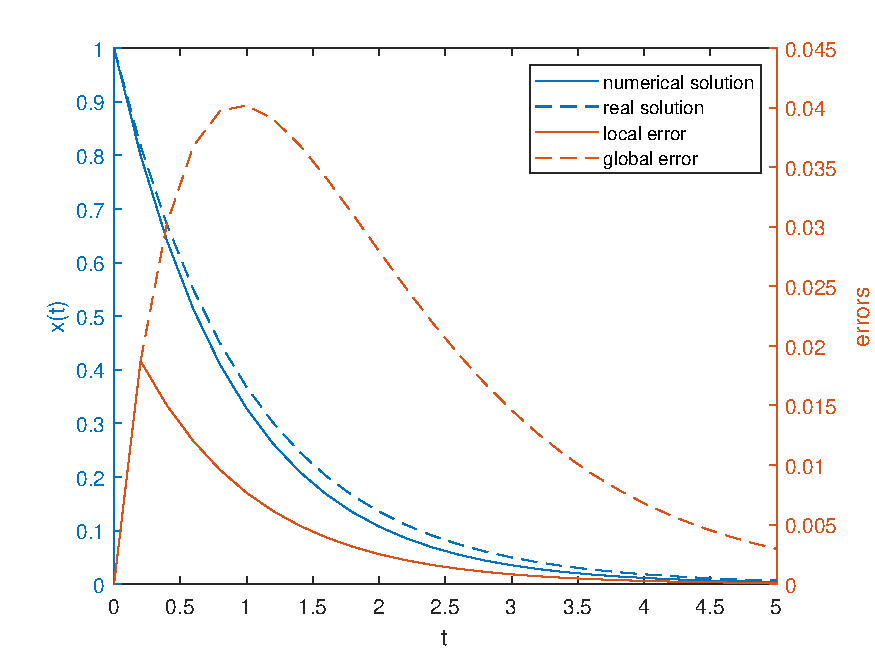
\includegraphics[width=\linewidth]{images/1/1_3_explicit_0_2.pdf} 
        \caption{Explicit Euler}
    \end{subfigure}%\hfill
    \begin{subfigure}{0.5\linewidth}
        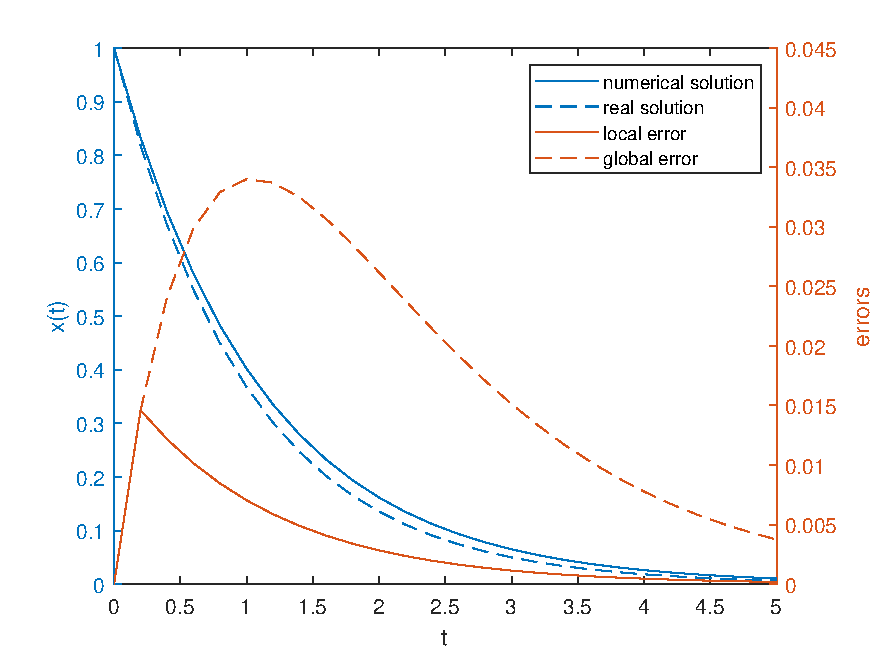
\includegraphics[width=\linewidth]{images/1/1_3_implicit_0_2.pdf}
        \caption{Implicit Euler}
    \end{subfigure}
    \caption{Local and global errors of the test equation}
    \label{1_3_errors}
\end{figure}

In these plots we can observe the two methods in action, and how they lend us a different result. For this particular time step size both the local and global error in the implicit Euler are lower than in the explicit one.

%%%%%%%%%%%%%%%%%%%%%%%%%%%%%%%%%%%%%%%%%%%%%%%%%%%%%%%%%%%%%%%%%%%%%%%%%%%%%%%%%%%%%%%%%%%%%%%%%%%

\subsection{Plot the local error vs the time step for the explicit Euler method and
the implicit Euler method. Does the plot behave as you would expect.
Explain what we mean by order. What is the order of the explicit Euler
method and the implicit Euler method, respectively. You should base your
answer on your numerical simulations. Is this as you would expect using
asymptotic theoretical considerations?} \label{1_4}

In Ascher-Petzold chapter 3.2 \cite{Ascher-Petzold} we find a definition of consistency of the method. We can find the order of consistency of these methods through the \textit{local truncation error}. In the book there's a derivation for the explicit Euler method that yields:
\begin{equation*}
    \mathbf{d}_n = \frac{h_n}{2}\mathbf{y}''(t_{n-1}) + \mathcal{O}(h_n^2).
\end{equation*}
Therefore, we can conclude the explicit Euler method is consistent of order 1. Using Dahlquist theorem \cite{Dahlquist_1956}, as the method is also zero-stable we know the method is convergent of order 1. Later in the chapter, the local error (here written as $\mathbf{l}_n$) is defined. Equation (3.14) in \cite{Ascher-Petzold} reads:
\begin{equation*}
    h_n|\mathcal{N}_h \hat{\mathbf{y}}(t_n)| = |\mathbf{l}_n|(1 + \mathcal{O}(h_n)).
\end{equation*}
We can therefore conclude that the local error will have order $1+1=2$.

We can follow a similar reasoning for obtaining the orders of the implicit Euler. We define the difference operator of the implicit Euler as:
\begin{equation*}
    \mathcal{N}_h u(t_n) = \frac{u(t_n) - u(t_{n-1})}{h_n} - f(t_n, u(t_n)).
\end{equation*}

Using Taylor's expansion $y(t_{n-1}) = y(t_n) - h_n y'(t_n) + \frac{h_n^2}{2}y''(t_n) + \ldots$ we get a local truncation error:
\begin{align*}
    \mathbf{d}_n &= \mathcal{N}_h y(t_n) = \frac{y(t_n) - y(t_{n-1})}{h_n} - f(t_n, y(t_n)) \\
    &= \frac{y(t_n) - \left[ y(t_n) - h_n y'(t_n) + \frac{h_n^2}{2}y''(t_n) + \mathcal{O}(h_n^3) \right]}{h_n} - y'(t_n) \\
    &= - \frac{h_n}{2}\mathbf{y}''(t_n) + \mathcal{O}(h_n^2).
\end{align*}
Therefore, we can conclude that the Implicit Euler is consistent of order 1. Notice that we get a different sign as in the explicit Euler, and this is completely consistent with what we see in figure \ref{1_3_errors}. As the implicit Euler is also zero-stable we know that the method is also convergent of order 1. Just as before, the local error should also scale with order 2 with the time step size.

Computing the mean of the local and the global error for the test equation with $\lambda=-1$, $x_0 = 1$, $\code{tspan}=[0, 20]$ and different time step sizes, ranging from $h=0.01$ to $0.5$ we finally obtain the results shown in Figure \ref{1_4_5_errors}. The local error escalates as a function of $h^2$ for both methods, just as what was expected from the mathematical derivation. 

\begin{figure}[h!]
\centering
    \begin{subfigure}{0.5\linewidth}
        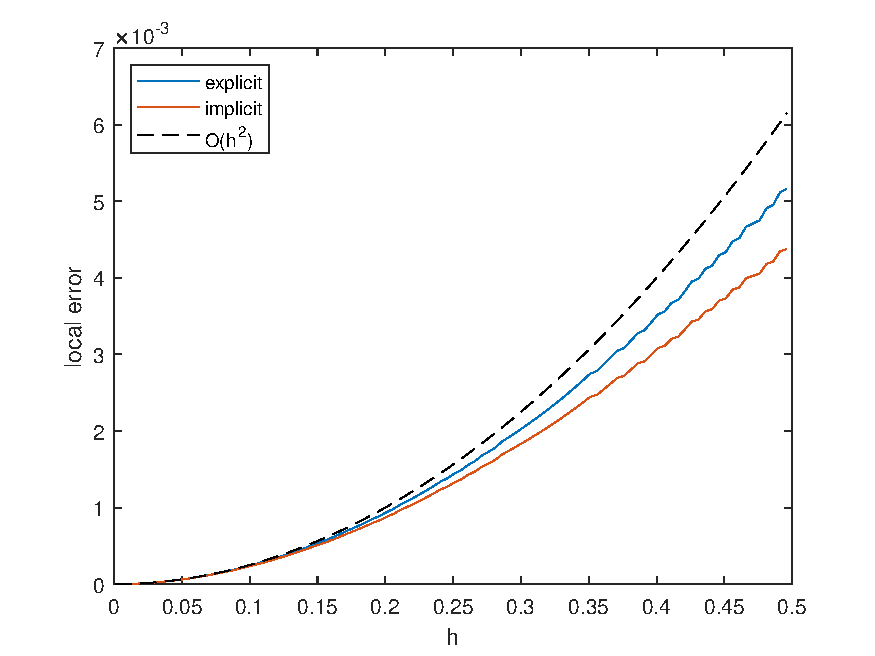
\includegraphics[width=\linewidth]{images/1/1_4_localerror.pdf} 
        \caption{Local Error}
    \end{subfigure}%\hfill
    \begin{subfigure}{0.5\linewidth}
        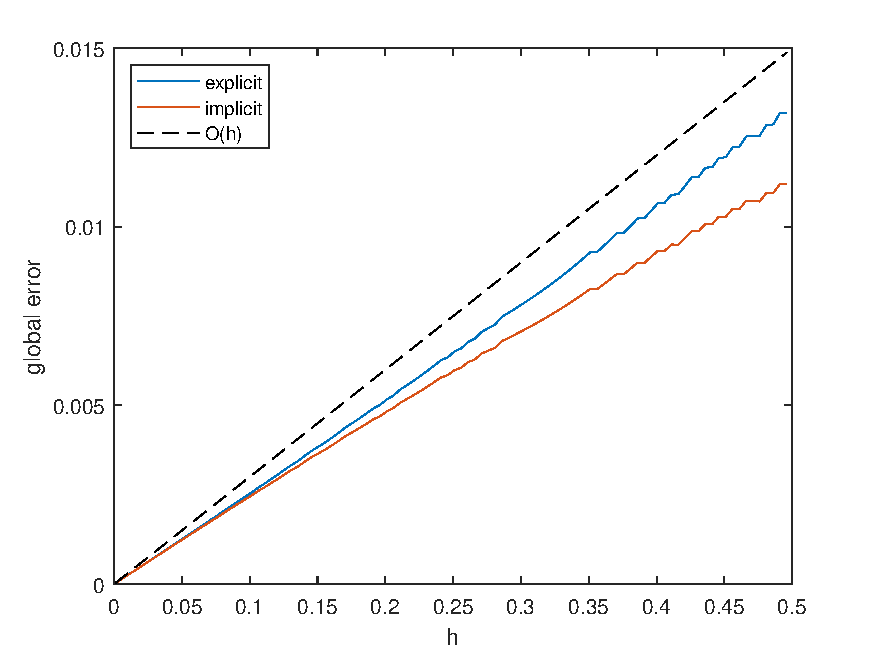
\includegraphics[width=\linewidth]{images/1/1_5_globalerror.pdf}
        \caption{Global Error}
    \end{subfigure}
    \caption{Errors of the Test Equation}
    \label{1_4_5_errors}
\end{figure}

%%%%%%%%%%%%%%%%%%%%%%%%%%%%%%%%%%%%%%%%%%%%%%%%%%%%%%%%%%%%%%%%%%%%%%%%%%%%%%%%%%%%%%%%%%%%%%%%%%%

\subsection{Plot the global error vs the time step for the explicit Euler method and
the implicit Euler method. Does the plot behave as you would expect.}
Following what we got in the previous exercise, as both methods have order 1 the global error should scale linearly with $h$. Taking a look at Figure \ref{1_4_5_errors}, we can see that the global error behaves as expected for both methods. It's also worth mentioning that the Implicit method has a lower local and global error for the test equation. This makes total sense if we analyze the expression of the local truncation error obtained in the previous exercise.

%%%%%%%%%%%%%%%%%%%%%%%%%%%%%%%%%%%%%%%%%%%%%%%%%%%%%%%%%%%%%%%%%%%%%%%%%%%%%%%%%%%%%%%%%%%%%%%%%%%

\subsection{Explain stability of a method and derive the expressions for the stability of
the explicit Euler method and the implicit Euler method. Plot the stability
regions. Explain A-stability. Is the explicit Euler-method A-stable? Is the
implicit Euler method A-stable?}

The concept of stability of a method comes from the concept of stability of a given problem. When looking at the Test Equation system in \ref{test_equation} (with $\lambda \in \mathbb{C}$), we can distinguish three different cases:
\begin{itemize}
    \item $\text{Re}(\lambda) > 0$, the solution grows exponentially with $t$ and the problem is \textit{unstable}. The distance between solution curves increases in time. In linear problems, the space of the solution (in this case $\mathbb{R}$) is then referred as the \textit{unstable space}
    \item $\text{Re}(\lambda) = 0$, the solution is either oscillating or 0, making the distance between solution curves to stay constant over time. This is referred as the \textit{center space}
    \item $\text{Re}(\lambda) < 0$, then the exponential decreases over time. The distance between curves decreases and the problem is \textit{asymptotically stable}. This yields an additional \textit{absolute stability} requirement:
    \begin{equation} \label{stability_requirement}
        |x_n| \leq |x_{n-1}|, \quad \forall n.
    \end{equation}
\end{itemize}

If we now take a look at how the Explicit Euler method is calculated iteratively for the Test Equation:
\begin{equation*}
    x_{n + 1} = x_n + h\lambda x_n = (1+h\lambda) x_n = (1+h\lambda)^2 x_{n-1} = \cdots = (1+h\lambda)^{n+1} x_0.
\end{equation*}
The only way \ref{stability_requirement} is going to be met is if:
\begin{equation*}
    |1+h\lambda| \leq 1.
\end{equation*}
This restricts the stability of the Explicit Euler to certain values of $h\lambda$. This region is depicted coloured in Figure \ref{stability_regions}.

For the Implicit Euler:
\begin{equation*}
     x_{n + 1} = x_n + h\lambda x_{n+1} = (1-h\lambda)^{-1} x_n = (1-h\lambda)^{-2} x_{n-1} = \cdots = (1-h\lambda)^{-(n+1)} x_0.
\end{equation*}
The stability condition in this case is:
\begin{equation*}
    \frac{1}{|1-h\lambda|} \leq 1.
\end{equation*}
This region is also depicted in Figure \ref{stability_regions}.

This leads us to the concept of A-Stability. A method is considered \textit{A-stable} if its region of absolute stability contains the entire left half-plane of $z=h\lambda$, i.e. $\text{Re}(h\lambda) < 0$. From Figure \ref{stability_regions} we can conclude that the Explicit Euler is not A-stable, while the Implicit Euler is.

\begin{figure}[h!]
\centering
    \begin{subfigure}{0.5\linewidth}
        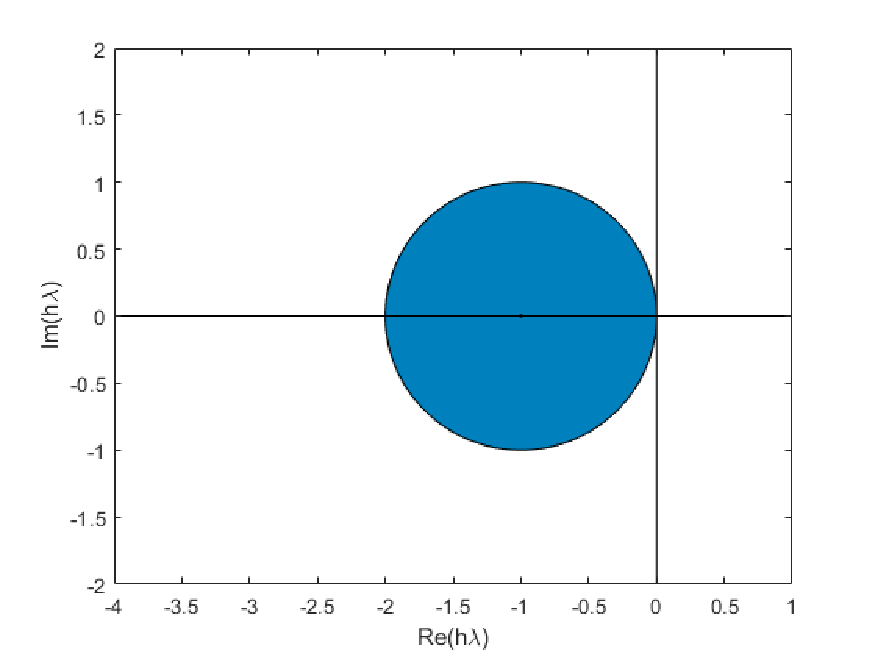
\includegraphics[width=\linewidth]{images/1/1_6_explicit.pdf} 
        \caption{Explicit Euler}
    \end{subfigure}%\hfill
    \begin{subfigure}{0.5\linewidth}
        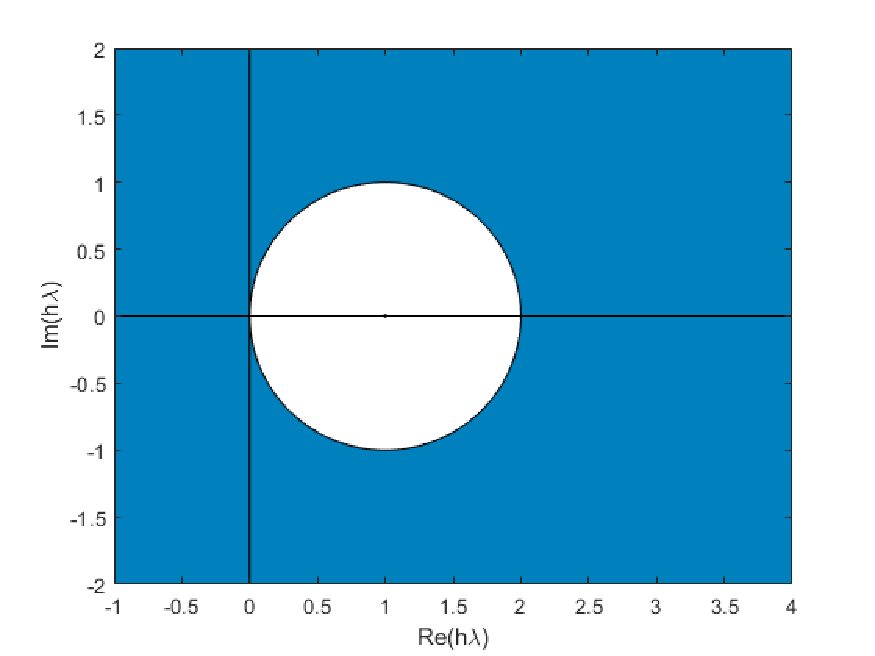
\includegraphics[width=\linewidth]{images/1/1_6_implicit.pdf}
        \caption{Implicit Euler}
    \end{subfigure}
    \caption{Absolute stability regions}
    \label{stability_regions}
\end{figure}